\documentclass[10pt,a4paper]{article}
\usepackage[margin=2.2cm]{geometry}
\usepackage[T1]{fontenc}
\usepackage{lmodern}
\usepackage{parskip}
\usepackage{booktabs}
\usepackage{tabularx}
\usepackage{array}
\usepackage{float}
\usepackage{graphicx}
\usepackage{enumitem}
\usepackage{xcolor}
\usepackage[colorlinks=true,urlcolor=blue!60!black,linkcolor=black]{hyperref}

\graphicspath{{../sig_bench_20261124_010231/figures/}}
\newcolumntype{R}{>{\raggedleft\arraybackslash}X}

\title{Drone Authentication Study --- Step 1 Progress Report\\[3pt]
\large Signature algorithms on the ESP32: RSA-3072, ECDSA P-256, Ed25519 and ML-DSA-44/65/87}
\author{}
\date{24 November 2026}

\begin{document}
\maketitle

\section*{Summary}

We measured six signature algorithms on one ESP32 in one firmware, under identical
conditions, 1,000 times each. The main results:

\begin{itemize}[nosep]
  \item \textbf{Ed25519 is the fastest} for one authentication (sign + verify: 29.2\,ms).
        \textbf{ML-DSA-44 is second} (68.2\,ms), and it is 5.5 times faster than RSA-3072
        (375.2\,ms) and 6.9 times faster than ECDSA P-256 (471.2\,ms).
  \item \textbf{ML-DSA signing time is not predictable.} The classical algorithms always take
        almost the same time (spread below 1\%). ML-DSA-44 signs in 54.7\,ms on median, but
        1 in 100 signatures takes more than 290\,ms and the slowest took 486\,ms. For a drone
        with fixed deadlines, this is the most important result.
  \item \textbf{ML-DSA's real costs are size and stack}, not speed: a 2,420-byte signature
        (Ed25519: 64 bytes) and 15--23\,KB of stack. It needs no heap memory at all.
  \item \textbf{Higher ML-DSA security costs about 2--3 times more}: ML-DSA-87 needs 2.5 times
        the signing time and 1.9 times the signature size of ML-DSA-44.
\end{itemize}

% ---------------------------------------------------------------------------
\section{What we measured and how}

The research question is which signature algorithm a drone should use to prove its identity.
We compare the classical algorithms used today with the post-quantum standard ML-DSA (NIST
FIPS 204), and the three ML-DSA security levels with each other.

\begin{table}[H]
\centering\small
\begin{tabularx}{\textwidth}{@{}l X@{}}
\toprule
Board & ESP32-D0WD (2 cores), CPU fixed at 240\,MHz, Wi-Fi and Bluetooth off \\
Software & Arduino core 3.3.12 (ESP-IDF 5.5.5), mbedTLS 3.6.6, libsodium 1.0.21,
           mldsa-native v1.0.0-beta2 \\
Algorithms & Ed25519 (libsodium); ECDSA P-256 and RSA-3072 with SHA-256 (mbedTLS); ML-DSA-44,
             ML-DSA-65, ML-DSA-87 (mldsa-native) \\
Runs & 1,000 key generations, signatures and verifications per algorithm (RSA key generation:
       30, as one takes 4--47\,s) \\
Messages & The same 1,000 messages (64 bytes, all different) for every algorithm \\
Timing & CPU cycle counter; each measurement in a fresh task on core 1; nothing printed while timing \\
\bottomrule
\end{tabularx}
\caption{Test setup.}
\end{table}

\textbf{How we made it fair.} All six algorithms run in \emph{one} firmware on \emph{one} board.
(Our two earlier benchmarks were separate programs and disagreed on Ed25519: 9.6\,ms and
15.9\,ms. This run gives 9.4\,ms and replaces both.) Signing and verifying always start from the
message, so for ECDSA and RSA the SHA-256 hash is included in the time. At the end, Ed25519 was
timed again: 9.426\,ms at the start and 9.437\,ms at the end (+0.1\%), so conditions stayed the
same for the whole 36-minute run.

\textbf{Correctness.} Before timing, every algorithm had to pass a known-answer test against an
independent implementation: Ed25519 against RFC 8032, ECDSA against RFC 6979 (the exact
signature), RSA against OpenSSL, and ML-DSA-44/65/87 against dilithium-py (byte-for-byte
identical keys and signatures). All six passed, and none of the 19,000 operations failed.

\textbf{One difference to keep in mind.} The ESP32 libraries use hardware for RSA and ECDSA
(big-number maths and SHA-256) and for the SHA-512 inside Ed25519. ML-DSA runs completely in
software. This is the default set-up, and it favours the classical algorithms.

% ---------------------------------------------------------------------------
\section{Time to authenticate}

\begin{figure}[H]
\centering
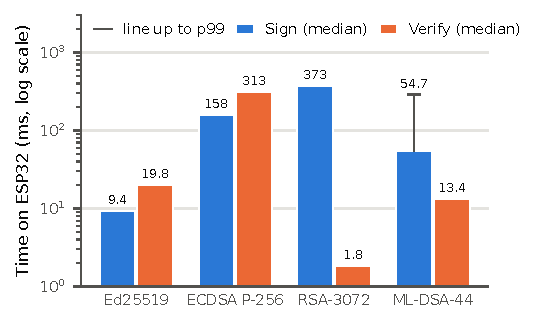
\includegraphics[width=0.62\textwidth]{fig1_auth_time.pdf}
\caption{Signing and verifying time (bar: median of 1,000 runs; line: up to the 99th
percentile). Log scale. Only ML-DSA-44 has a visible spread.}
\end{figure}

\begin{table}[H]
\centering\small
\begin{tabularx}{\textwidth}{@{}l RRRR RRRR@{}}
\toprule
 & \multicolumn{4}{c}{\textbf{Sign (ms)}} & \multicolumn{4}{c}{\textbf{Verify (ms)}} \\
\cmidrule(lr){2-5}\cmidrule(l){6-9}
Algorithm & Median & p95 & p99 & Max & Median & p95 & p99 & Max \\
\midrule
Ed25519     & 9.43   & 9.44   & 9.44   & 9.44     & 19.79  & 20.05  & 20.14  & 20.23 \\
ECDSA P-256 & 158.18 & 158.56 & 158.69 & 158.88   & 313.07 & 313.40 & 313.51 & 313.63 \\
RSA-3072    & 373.44 & 375.63 & 376.50 & 377.77   & 1.81   & 1.84   & 1.85   & 1.87 \\
ML-DSA-44   & 54.74  & 198.38 & 289.51 & 486.00   & 13.44  & 13.44  & 13.44  & 13.44 \\
ML-DSA-65   & 103.61 & 419.66 & 681.15 & 1,110.78 & 22.48  & 22.48  & 22.48  & 22.48 \\
ML-DSA-87   & 137.96 & 525.29 & 769.46 & 1,170.08 & 38.76  & 38.76  & 38.76  & 38.76 \\
\bottomrule
\end{tabularx}
\caption{Signing and verifying time, 1,000 runs each. p95/p99: 95\%/99\% of runs were faster.}
\end{table}

\begin{itemize}[nosep]
  \item \textbf{Sign + verify (medians):} Ed25519 29.2\,ms, ML-DSA-44 68.2\,ms, ML-DSA-65
        126.1\,ms, ML-DSA-87 176.7\,ms, RSA-3072 375.2\,ms, ECDSA P-256 471.2\,ms.
  \item \textbf{ML-DSA verifies quickly and always in the same time}; ML-DSA-44 verifies faster
        than Ed25519 (13.4 vs 19.8\,ms). This helps the side that checks many drones.
  \item \textbf{RSA-3072 verifies fastest} (1.8\,ms) but signs slowest (373\,ms), which is a poor
        fit for a drone, because the drone is the side that signs.
\end{itemize}

% ---------------------------------------------------------------------------
\section{ML-DSA signing time is not predictable}

\begin{figure}[H]
\centering
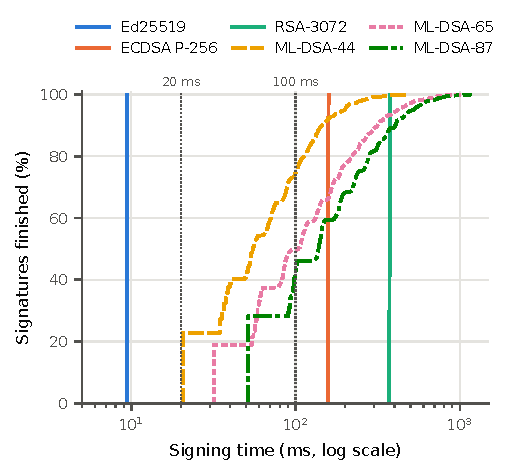
\includegraphics[width=0.62\textwidth]{fig2_sign_cdf.pdf}
\caption{Share of the 1,000 signatures that finished within a given time. A vertical line means
the algorithm always takes the same time. Dotted lines: example drone deadlines of 20 and 100\,ms.}
\end{figure}

ML-DSA builds a candidate signature and throws it away if releasing it could leak information
about the secret key, then tries again. The number of tries changes from message to message,
which is why its curves rise in steps (each step is most likely one more try) and have long
tails. The classical algorithms are vertical lines: every signature takes the same time.

\begin{table}[H]
\centering\small
\begin{tabularx}{0.75\textwidth}{@{}l RRRR@{}}
\toprule
Algorithm & $>$ 20\,ms & $>$ 50\,ms & $>$ 100\,ms & $>$ 200\,ms \\
\midrule
Ed25519     & 0\%   & 0\%    & 0\%    & 0\% \\
ECDSA P-256 & 100\% & 100\%  & 100\%  & 0\% \\
RSA-3072    & 100\% & 100\%  & 100\%  & 100\% \\
ML-DSA-44   & 100\% & 58.5\% & 25.6\% & 5.0\% \\
ML-DSA-65   & 100\% & 81.1\% & 50.4\% & 22.7\% \\
ML-DSA-87   & 100\% & 100\%  & 57.1\% & 31.8\% \\
\bottomrule
\end{tabularx}
\caption{Share of signatures slower than a deadline (1,000 signatures each).}
\end{table}

For a drone this means: with ML-DSA, the authentication time must be planned for the slow cases,
not the average. For example, 1 in 4 ML-DSA-44 signatures takes more than 100\,ms.

% ---------------------------------------------------------------------------
\section{The three ML-DSA levels}

\begin{figure}[H]
\centering
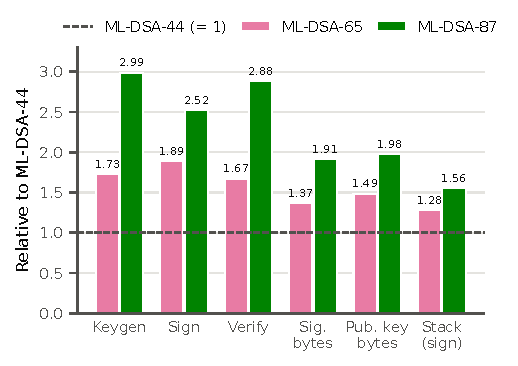
\includegraphics[width=0.62\textwidth]{fig3_mldsa_levels.pdf}
\caption{Cost of ML-DSA-65 (NIST category 3) and ML-DSA-87 (category 5) relative to ML-DSA-44
(category 2). Times are medians.}
\end{figure}

Going from ML-DSA-44 to ML-DSA-87 costs about 2.5--3 times more time and about 2 times more bytes.
Signing grows less than key generation and verifying. FIPS 204 expects ML-DSA-87 to need fewer
tries on average than ML-DSA-65 (we did not count the tries ourselves). All three levels need
almost the same flash (about 14\,KB), because they run the same code with different parameters.

% ---------------------------------------------------------------------------
\section{Key generation, sizes and memory}

\begin{table}[H]
\centering\small
\begin{tabularx}{\textwidth}{@{}l RRR RRR@{}}
\toprule
 & \multicolumn{3}{c}{\textbf{Key generation (ms)}} & \multicolumn{3}{c}{\textbf{Size (bytes)}} \\
\cmidrule(lr){2-4}\cmidrule(l){5-7}
Algorithm & Median & p95 & Max & Public key & Secret key & Signature \\
\midrule
Ed25519     & 8.02      & 8.03      & 8.03      & 32    & 64    & 64 \\
ECDSA P-256 & 145.98    & 146.22    & 146.39    & 65    & 32    & 69--72 \\
RSA-3072    & 12,929.42 & 28,277.26 & 46,896.90 & 384   & 1,767 & 384 \\
ML-DSA-44   & 13.06     & 13.06     & 13.06     & 1,312 & 2,560 & 2,420 \\
ML-DSA-65   & 22.53     & 22.54     & 22.54     & 1,952 & 4,032 & 3,309 \\
ML-DSA-87   & 39.01     & 39.01     & 39.01     & 2,592 & 4,896 & 4,627 \\
\bottomrule
\end{tabularx}
\caption{Key generation (done once, when the drone is set up) and sizes. RSA key generation: 30
runs. RSA public key: the 384-byte modulus (the exponent 65537 is fixed).}
\end{table}

\begin{table}[H]
\centering\small
\begin{tabularx}{\textwidth}{@{}l RRR RRR R@{}}
\toprule
 & \multicolumn{3}{c}{\textbf{Peak stack (bytes)}} & \multicolumn{3}{c}{\textbf{Peak heap (bytes)}} & \\
\cmidrule(lr){2-4}\cmidrule(lr){5-7}
Algorithm & Keygen & Sign & Verify & Keygen & Sign & Verify & \textbf{Flash} \\
\midrule
Ed25519     & 1,072  & 1,504  & 3,344  & 0     & 0     & 0     & 22,620 \\
ECDSA P-256 & 1,488  & 2,032  & 1,568  & 2,680 & 2,952 & 3,108 & 24,580 \\
RSA-3072    & 1,732  & 1,120  & 692    & 4,576 & 7,932 & 1,920 & 39,088 \\
ML-DSA-44   & 13,408 & 14,960 & 11,280 & 0     & 0     & 0     & 14,084 \\
ML-DSA-65   & 16,480 & 19,168 & 12,368 & 0     & 0     & 0     & 13,808 \\
ML-DSA-87   & 20,576 & 23,264 & 14,672 & 0     & 0     & 0     & 14,052 \\
\bottomrule
\end{tabularx}
\caption{Memory per operation and flash added to the firmware. The stack meter was checked with
a 16,384-byte test array, measured as 16,196 bytes (accurate to about 0.2\,KB).}
\end{table}

ML-DSA needs 15--23\,KB of stack but no heap; the mbedTLS algorithms need 3--8\,KB of heap. The
ESP32 has about 275\,KB of free memory, so every algorithm fits. (Our older benchmark reported
34.8\,KB of stack for ML-DSA-44; it used an earlier version of the library, so this new value
replaces it.)

% ---------------------------------------------------------------------------
\section{Limits and next steps}

\textbf{Limits.} One ESP32 board and one library per algorithm; ML-DSA without the hardware help
the classical algorithms get; no energy measurement (no power meter available); the RSA key
generation numbers come from 30 runs only.

\textbf{Next steps.}
\begin{enumerate}[nosep]
  \item How time grows with message size, and the largest message the ESP32 can sign.
  \item The authentication messages on the network, captured with Wireshark.
  \item Sequence diagrams for the drone authentication process.
  \item MPU6050 sensor on the ESP32: signed drone telemetry, and whether signing disturbs the
        sensor sampling.
\end{enumerate}

All code, raw measurements and scripts are in the project repository, in
\texttt{Drone\_Auth\_Research/}. Every number above is regenerated from the raw log by the
scripts.

\end{document}
